%%%%%%%%%%%%%%%
%
% $Autor: Wings $
% $Datum: 2020-01-29 07:55:27Z $
% $Pfad: General/ServoDrive.tex
% $Version: 1785 $
%
%
%%%%%%%%%%%%%%%

	
\chapter{Servomotor JAMRA 033212}

\Mynote{Ausfühtlicher!\\ Arduino-Programm? Genauigkeit?}



Elektromotoren besitzen bei geringen Drehzahlen eine geringe Kraftentfaltung. Um Platz zu sparen, werden deshalb Getriebe verwendet. Die hohe Motordrehzahl wird in ein langsames, aber hohes Drehmoment übersetzt. Dadurch bekommen Servomotoren ihre besonderen Eigenschaften: Sehr genaue Positions- und Geschwindigkeitsregelung. \cite{Bernstein:2018} 

\bigskip

Unterteilt werden Servomotoren in zwei Kategorien: Open Loop und Closed Loop. Der Open Loop-Motor hat keine Begrenzung im Drehwinkel und kann sich um $360^\circ$ frei drehen. Dieser wird auch als Schrittmotor bezeichnet. Die realisierte Anwendung zur Sonnennachführung benötigt jedoch keine volle Kreisbahn, weshalb der ausgewählte Motor in die Kategorie Closed Loop fällt. Die in der Industrie eingesetzten Servomotoren besitzen nicht zwingend ein Getriebe, sind daher deutlich größer als ein Modellbauservo. Basierend auf einem Brushless-Motor ist Magnet und Spule sehr groß ausgelegt, um die Kräfte aufzubauen. \Mynote{Quelle fehlt!} 

\bigskip

Bei dem verwendeten Servomotor ist das Chassis aus eingefärbtem, durchsichtigem Kunststoff gefertigt, weshalb ein Blick den Aufbau und die wesentlichen Bauteile zeigt.

\begin{figure}
    \begin{flushleft}
        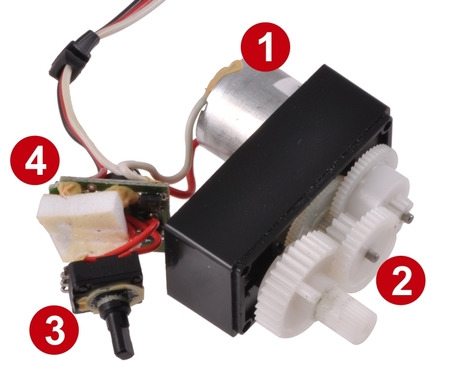
\includegraphics[width=10cm]{Drive/Servomotor}
        \caption{Aufbau eines Servomotors \href{https://a.pololu-files.com/picture/0J3188.450.jpg?8db0bf79b0d26db613e6730cedbc62f7}{Quelle}}
        \Mynote{Eigene Beschriftung mit overpic}
    \end{flushleft}
\end{figure}



\begin{description}
  \item[Motor:] Als Aktuator ist im JAMRA 033212 ein Gleichstrommotor verbaut. Da der Motor in der Baugruppe das schwerste Bauteil ist, muss je nach Anwendung aus Einsatzzweck und Realisierung durch Getriebe und Motor ein korrektes Verhältnis abgeleitet werden. In der Sonnennachführung verläuft die Hauptlast vertikal nach unten und wird dort gelagert. Der Servomotor muss also nur ein vergleichsweise geringes Drehmoment aufbringen.

  \item[Getriebe:] Um bei kleinen Motoren das notwendige Drehmoment aufzubringen, wird ein mehrstufiges Getriebe mit hoher Untersetzung eingesetzt. Bei hochwertigen, teuren Servomotoren besteht das Getriebe aus Metallzahnrädern und ist kugelgelagert, der vorhandene Servomotor besitzt ein kostensparendes Kunststoffgetriebe.

  \item[Positionssensor:] Bei dem Servomotor ist an der Ausgangswelle ein Potentiometer angebracht. Ein Potentiometer ist ein verstellbarer Widerstand welcher als Spannungsteiler ausgelegt ist.  Bei Drehung der Welle um einen bestimmten Winkel wird der Widerstand des Potentiometers verändert. Das mittlere Anschlussbein ist der Wischer, welcher am Schleifring entlang schleift. 

  \item [Motorsteuerung:] In der Motor Steuerung kommen Spannung, Position und externes Steuersignal zusammen. Geregelt wird abhängig von der Last die Spannung und von der externen Steuerung die Position. Unterschiede gibt es in Analog- und Digitaler Steuerung. Bei der digitalen Steuerung ist ein zusätzlicher Mikrocontroller verbaut welcher die Position exakter anfahren und halten kann. Dieser ist jedoch auch teurer, weshalb wir uns für die analoge Ausführung entschieden haben.
  
  Die Spannung aus dem Spannungsteiler (Potentiometer) wird mit der Spannung aus dem Impulswandler verglichen. Aus dem Impulswandler kommt das veränderte Signal vom Arduino. Das Signal vom Arduino kommt über eine Signalleitung mit 50 Hz. Je nachdem wie breit das Signal ist, kann die Winkelstellung durch den Motor Treiber verändert werden. Die Änderung der Signalbreite wird auch als Puls Weiten Modulation bezeichnet, kurz PWM. \cite{Dejan:2018,Ibrahim:2018}
  
  Dadurch ist es möglich den Servomotor mit nur einer Steuerleitung anzusteuern. Bei steigender Spannung erhöht sich das Impulssignal bei gleichbleibender Breite. Der Servomotor ändert mit höherer Spannung seine Position schneller und auch die Stellkraft steigt. Beim Halten der Position ist der Stromverbrauch sehr gering, weshalb Servomotoren auch als Verstelleinheit eingesetzt werden.

  \begin{figure}
    \begin{center}
        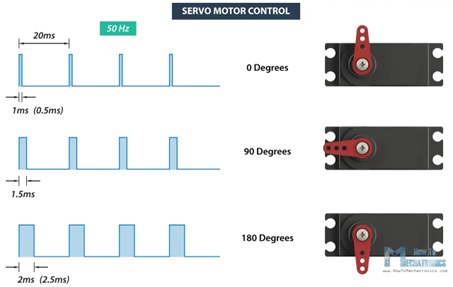
\includegraphics[width=14cm]{Drive/ServoPMW}
        \caption{PWM am Servomotor \href{https://howtomechatronics.com/wp-content/uploads/2018/03/RC-Servo-Motor-Control-Signal-768x485.png?ezimgfmt=ng:webp/ngcb2}{Quelle}}
    \end{center}\Mynote{keine geeignete Quelle, richtig zitieren; eigene Zeichnung moit tikz}
  \end{figure}

\end{description}


\section{Datenblatt JAMRA 033212} 

Die Zusatzbezeichnung 9g bezieht sich auf das Eigengewicht, welches ungefähr 9 Gramm beträgt und die Bauklasse kennzeichnet. Zum Beispiel im Flugzeugmodellbau als Klappen-oder Fahrwerkssteuerung. Wichtig ist für die Anwendung vor allem die Stellkraft. Im Vorfeld muss die aufzubringende Kraft bekannt sein, um einen Passenden Servomotor auszuwählen. Am Datenblatt wird nochmal deutlich was bei steigender Spannung passiert. Die Kraft und die Geschwindigkeit nehmen zu. Den einfachen, günstigen Servomotor erkennt man auch am Kunststoffgetriebe und an fehlenden Kugellagern.

\begin{figure}
  \begin{center}
    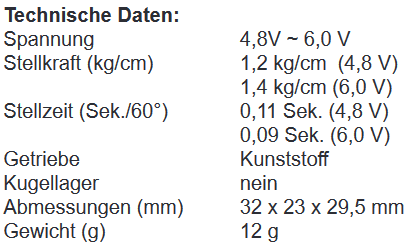
\includegraphics[width=12cm]{Drive/ServoDataSheet}
    \caption{Auszug aus Gebrauchsanleitung JAMRA 033212, Seite 1 \cite{Jamara:2018}}
  \end{center}\Mynote{Informationen herausziehen, eigene Tabelle}
\end{figure}



\section{Schaltplan}

\begin{figure}
    \begin{center} 
        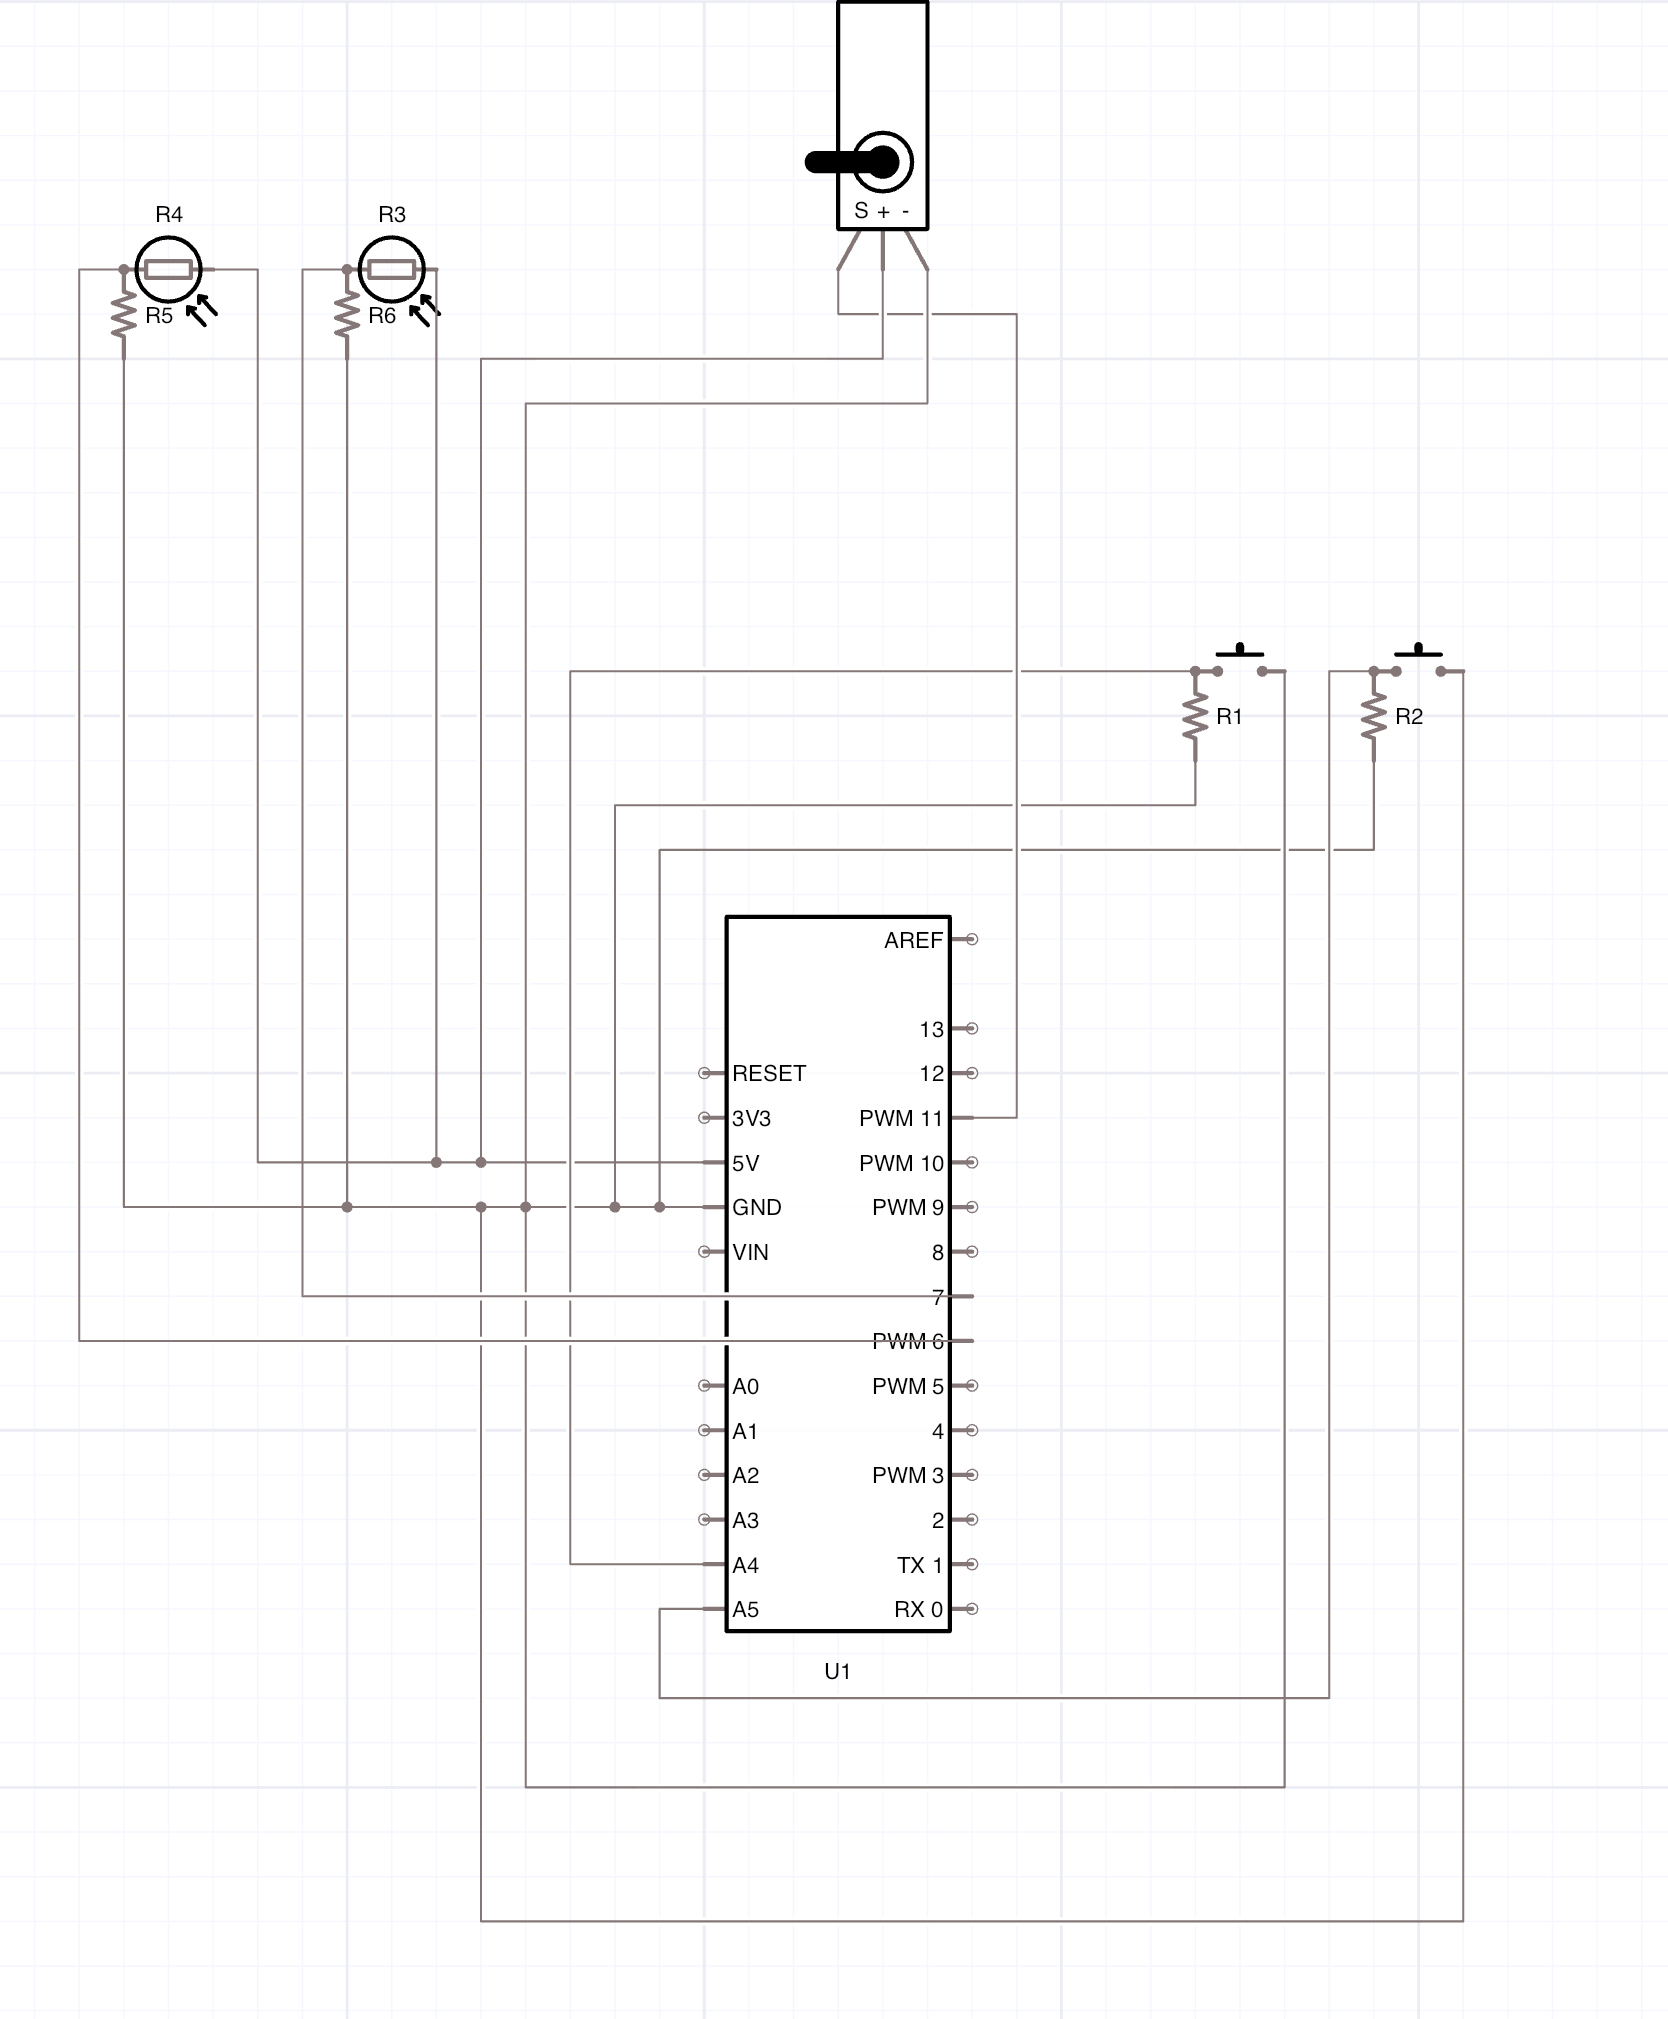
\includegraphics[width=14cm]{Drive/ServoCircuit}
        \caption{Schaltplan zum Anschluss eines Servomotors JAMRA 033212}\Mynote{Wo ist das Grove-Kabel? Motherboard?}
    \end{center} 
\end{figure}
